 % 五号字体,开明式标点处理,不设置默认字体
\documentclass[UTF8,12pt,punct=kaiming,fontset=none]{article}
\usepackage[UTF8]{ctex}
\usepackage{fontspec}
\usepackage{tikz}
\usepackage{graphicx}
\usepackage{subcaption}
\usepackage{pgf-umlsd}
% 品红色链接和注释
% \usepackage[colorlinks=true, linkcolor=magenta, citecolor=magenta, urlcolor=magenta]{hyperref}
% 黑色链接和注释
\usepackage[colorlinks=true, linkcolor=black, citecolor=black, urlcolor=black]{hyperref}
\usepackage{geometry}
\usepackage{fancyhdr}
\usepackage{multirow}
\usepackage{boldline}
\usepackage[european,nooldvoltagedirection]{circuitikz}
\usepackage{titlesec}
\usepackage{caption}
\usepackage{floatrow}
\usepackage{amssymb}

% 字体
\IfFontExistsTF{Source Han Serif SC}
{
    \setCJKmainfont{Source Han Serif SC}
}
{
    % GitHub Actions
    \setCJKmainfont[
        Path=../fonts/ ,
        Extension = .otf ,
        UprightFont = *-Regular ,
        BoldFont = *-Bold
    ]{SourceHanSerifSC}
}
\IfFontExistsTF{Source Han Sans SC}
{
    \setCJKsansfont{Source Han Sans SC}
}
{
    % GitHub Actions
    \setCJKsansfont[
        Path=../fonts/ ,
        Extension = .otf ,
        UprightFont = *-Regular ,
        BoldFont = *-Bold
    ]{SourceHanSerifSC}
}
\IfFontExistsTF{DejaVu Sans}
{
    \newfontfamily\ds{Computer Modern}
}
{
    % GitHub Actions
    \newfontfamily\ds[
        Path=. ./fonts/ ,
        Extension = . ttf ,
        BoldFont = *-Bold ,
        ItalicFont = *-Oblique ,
        BoldItalicFont = *-BoldOblique
    ]{DejaVuSans}
}
\newfontfamily\cm{Computer Modern}

% 布局
\geometry{a4paper,left=2cm,right=2cm,top=2.5cm,bottom=2.5cm}
\setlength{\headheight}{25pt}

% 图表标题
\DeclareCaptionFont{captionfont}{\ds\small}
\captionsetup{font=captionfont}
\floatsetup{style=plaintop}

% 页眉页脚
\pagenumbering{arabic}
\pagestyle{fancy}
\fancyhead[L]{\ds · \hspace{0.1cm} \thepage \hspace{0.1cm} ·}
\fancyhead[C]{\ds 红石数电评论\\\scriptsize{Review of Redstonic Digital Circuit}}
\fancyhead[R]{\ds 2022年1月(第1期)}
\fancyfoot[L,C,R]{}

% 标题
\title{\vspace{-1.5cm}基于基本红石电路的函数绘图显示器\vspace{-0.5cm}}
\author{\ds @章鱼千\hspace{-0.015cm}\_zhyq\footnote{\ds Bilibili id: 287032573}}
\date{}

% 参考文献标注
\newcommand*{\upcite}[1]{
    \ds\textsuperscript{\cite{#1}}\cm
}

\begin{document}
    \maketitle
    \thispagestyle{fancy} % 首页页眉页脚
    \vspace{-0.7cm}

    % 摘要及关键词
    \begin{flushright}
        \begin{minipage}[c]{0.91\linewidth}
            \titleformat{\section}[leftmargin]{\sffamily\small\bfseries}{}{0cm}{}
            \titlespacing{\section}{1.5cm}{1ex}{0cm}

            \section{摘 \hspace{0.105cm} 要}
            \ds \small 本文介绍了一种基于基本红石电路的函数绘图显示器,其基本功能是根据设置好的各个点的坐标在显示器中绘制函数图像.文中首先介绍了显示器的整体组成与各部分的功能,然后依次介绍了各个部分的具体原理.最终的成品如 BV17K4y1a7ip 所示.

            \section{关键词}
            \ds \small 基本红石电路 \hspace{0.5cm} 函数绘图 \hspace{0.5cm} 显示器 \hspace{0.5cm} 存储器
        \end{minipage}
    \end{flushright}
    \vspace{0.2cm}

    % 节标题格式
    \titleformat{\section}[hang]{\large\sffamily\bfseries}{\textmd{\ds\thesection}}{0.5cm}{}
    \titlespacing{\section}{0cm}{0.5ex}{0.2ex}
    \titleformat{\subsection}[hang]{\normalsize\sffamily}{\textmd{\ds\thesubsection}}{0.5cm}{}
    \titlespacing{\subsection}{0cm}{0.5ex}{0.2ex}
    \setcounter{section}{-1}

    \section{引言}
    受限于我的世界的游戏机制,不依靠指令在原版游戏中建造通用显示器是非常困难的.据笔者所知,目前我的世界中的显示器作品都只能实现部分功能,例如字符显示器\upcite{bib:1}\upcite{bib:2}可以实现打字功能、视频播放器\upcite{bib:3}可以依次播放存储于只读存储器中的图像与七段式数码管\upcite{bib:4}用于显示数字等.

    本文介绍了一种基于基本红石电路的函数绘图显示器,其基本功能是根据设置好的各个点的坐标在显示器中绘制函数图像.如果接入计算元件,也可以显示计算元件得到的函数图像,例如\cite{bib:5}中利用加法器计算一次函数图像等.

    基本红石电路是指利用建筑材料、红石粉、红石中继器、红石火把和少量活塞的电路.通常来说,很可能可以通过在这类电路中引入其他元件来优化体积与延时,尽管如此,由于这类电路的逻辑相对清晰易懂,因此对于初学者来说通过这类电路学习数电工程的构建方法依然是很有意义的.

    本文首先介绍函数绘图显示器的总体结构与各个部分的功能,然后以一个$4 \times 4$的显示器为例依次介绍各个部分的组成,最后将介绍$32 \times 32$的样机,更详细的样机展示见\ds BV17K4y1a7ip\cm .

    \section{总体结构与功能}
    本文介绍的函数显示器主要包括三部分:显示器、存储器与总控电路,三部分的输入输出及其含义如表 \ref{tab:1} 所示,连接图如图 \ref{fig:1} 所示.

    \begin{figure}[H]
        \begin{floatrow}
            \ttabbox
            {
                \caption{显示器各部分的输入输出与含义}
                \label{tab:1}
            }
            {
                \scalebox{0.8}{\begin{tabular}{c c c}
                \hlineB{3}
                模块 & 输入输出 & 含义 \\
                \hlineB{3}
                \multirow{5}{*}{\centering 显示器} & 显示器输出 & 为用户输出图像 \\
                \cline{2-3}
                & 行输入 & \multirow{3}{5cm}{\centering 当输入选择信号激活时,行、列输入信号对应的点会被激活} \\
                \cline{2-2}
                & 列输入 & \\
                \cline{2-2}
                & 输入选择 &  \\
                \cline{2-3}
                & 清零 & 熄灭显示器上的所有像素 \\
                \hline
                \multirow{2}{2cm}{\centering 存储器} & 地址输入 & \multirow{2}{5cm}{\centering 输出存储器中地址对应位置存储的信息} \\
                \cline{2-2}
                & 存储输出 & \\
                \hline
                总控电路 & 控制信号 & \\
                \hlineB{3}
                \end{tabular}}
            }
            \ffigbox
            {
                \caption{函数显示器的总体结构}
                \label{fig:1}
            }
            {
                \scalebox{0.8}{\begin{circuitikz}[line width=0.8pt]
                \ctikzset{multipoles/thickness=2}
                \ctikzset{chips/scale=1.2}
                \draw (0,0) node[qfpchip, num pins=12, hide numbers, no topmark, external pins width=0](C1){显示器};
                \draw (7,0) node[qfpchip, num pins=12, hide numbers, no topmark, external pins width=0](C2){存储器};
                \draw (0,-4) node[qfpchip, num pins=12, hide numbers, no topmark, external pins width=0](C3){控制器};
                \draw (C1.bpin 4) to[short, -, l=清零] (C3.bpin 12);
                \draw (C1.bpin 6) to[short, -, l=显示器时钟] (C3.bpin 10);
                \draw (C1.bpin 7) to[short, -, l=行选择(二进制)] (C2.bpin 3);
                \draw (C1.bpin 9) to[short, -, l=列选择(二进制)] (C2.bpin 1);
                \draw (C3.bpin 8) to[short, -, l=存储器时钟] (7,-4) -- (C2.bpin 5);
                \end{circuitikz}}
            }
        \end{floatrow}
    \end{figure}

    在下面各部分中,我们将会分别介绍三部分的具体结构与建造方法.

    \section{显示器}
    \subsection{显示器结构}
    显示器的结构图如图 \ref{fig:2} 所示,其输入包括显示器清零信号、输入控制信号、行选择信号与列选择信号.其中显示器清零信号的功能是在激活时熄灭显示器中的所有像素,输入控制信号激活时会根据行选择信号、列选择信号的值点亮相应的像素.

    \begin{figure}[H]
        \scalebox{0.8}{\begin{circuitikz}[line width=0.8pt]
        \ctikzset{multipoles/thickness=2}
        \ctikzset{chips/scale=0.8}
        \draw (0,0) node[dipchip, num pins=14, hide numbers, no topmark, external pins width=0, rotate=90](U1){\rotatebox{-90}{显示单元(1,1)}};
        \draw (0,-2) node[dipchip, num pins=14, hide numbers, no topmark, external pins width=0, rotate=90](U2){\rotatebox{-90}{显示单元(1,2)}};
        \draw (0,-3.5) node{$\ldots$};
        \draw (0,-5) node[dipchip, num pins=14, hide numbers, no topmark, external pins width=0, rotate=90](UN){\rotatebox{-90}{显示单元(N,N)}};
        \draw (5,0) node[dipchip, num pins=10, hide numbers, no topmark, external pins width=0, rotate=90](RS1){\rotatebox{-90}{RS锁存器}};
        \draw (5,-2) node[dipchip, num pins=10, hide numbers, no topmark, external pins width=0, rotate=90](RS2){\rotatebox{-90}{RS锁存器}};
        \draw (5,-3.5) node{$\ldots$};
        \draw (5,-5) node[dipchip, num pins=10, hide numbers, no topmark, external pins width=0, rotate=90](RSN){\rotatebox{-90}{RS锁存器}};
        \draw (15,0) node[dipchip, num pins=8, hide numbers, no topmark, external pins width=0, rotate=90](D1){\rotatebox{-90}{译码器}};
        \draw (15,-2) node[dipchip, num pins=8, hide numbers, no topmark, external pins width=0, rotate=90](D2){\rotatebox{-90}{译码器}};
        \ctikzset{chips/scale=1.5}
        \draw (10,-2.5) node[dipchip, num pins=16, hide numbers, no topmark, external pins width=0](AND){与门网络};
        \draw (U1.s) to[short, -, l=显示信号] (RS1.n);
        \draw (U2.s) to[short, -, l=显示信号] (RS2.n);
        \draw (UN.s) to[short, -, l=显示信号] (RSN.n);
        \draw (RS1.s) ++(0,0.2) node(RS11){};
        \draw (RS2.s) ++(0,0.2) node(RS21){};
        \draw (RSN.s) ++(0,0.2) node(RSN1){};
        \draw (RS1.s |- RS11) -- ++(0.4,0) to[short, -, l={\parbox{5cm}{\centering 置1信号\\ (1,1) \vspace{0.5cm}}}] (AND.w |- RS11);
        \draw (RS2.s |- RS21) -- ++(0.4,0) to[short, -, l={\parbox{5cm}{\centering 置1信号\\ (1,2) \vspace{0.5cm}}}] (AND.w |- RS21);
        \draw (RSN.s |- RSN1) -- ++(0.4,0) to[short, -, l={\parbox{5cm}{\centering 置1信号\\ (N,N) \vspace{0.5cm}}}] (AND.w |- RSN1);
        \draw (RS1.s) ++(0,-0.2) node(RS12){};
        \draw (RS2.s) ++(0,-0.2) node(RS22){};
        \draw (RSN.s) ++(0,-0.2) node(RSN2){};
        \draw (RS1.s |- RS12) -- ++(0.3,0) -- ++(0, -2);
        \draw (RS2.s |- RS22) -- ++(0.3,0) -- ++(0, -3);
        \draw (RSN.s |- RSN2) -- ++(0.3,0) -- ++(0, -1.5);
        \draw (RS2.s |- RS22) ++(0.3,0) node[circ]{};
        \draw (RSN.s |- RSN2) ++(0.3,0) node[circ]{};
        \draw (RSN.s |- RSN2) ++(1.5,-1) node{置0信号};
        \draw (AND.e |- D1.n) to[short, -, l={\parbox{5cm}{\centering 行选择\\ (独热码) \vspace{0.5cm}}}] (D1.n);
        \draw (AND.e |- D2.n) to[short, -, l={\parbox{5cm}{\centering 列选择\\ (独热码) \vspace{0.5cm}}}] (D2.n);
        \draw (D2.n) ++(0,-2) node(C){};
        \draw (AND.e |- C) to[short, -, l={\parbox{5cm}{\centering 输入控制\\ 显示器时钟 \vspace{0.5cm}}}] (D2.n |- C);
        \draw (D1.s) to[short, -, l={\parbox{5cm}{\centering 行选择\\ (二进制) \vspace{0.5cm}}}] ++(2.5,0);
        \draw (D2.s) to[short, -, l={\parbox{5cm}{\centering 列选择\\ (二进制) \vspace{0.5cm}}}] ++(2.5,0);
        \end{circuitikz}}
        \caption{显示器的结构}
        \label{fig:2}
    \end{figure}

    不失一般性地,我们讨论一个含有$N \times N$个像素的显示器,则显示器中的任意一个点的坐标可以用两个$n$位二进制数表示,其中$n$满足
    $$2^n \leqslant N < 2^{n+1}$$
    也就是显示器中行选择信号与列选择信号各包括$n$位信号.

    \subsection{基本显示单元}
    基本显示单元利用单路红石输入控制四个红石灯,当输入为激活时红石灯亮起.基本显示单元在我的世界中的建造方法如图 \ref{fig:3} 所示,图 \ref{fig:3b} 中左侧的橙色方块与图 \ref{fig:3a} 中右侧的黑色方块分别为点亮与熄灭的红石灯.

    \begin{figure}[H]
        \centering
        \begin{subfigure}{0.2\linewidth}
            \centering
            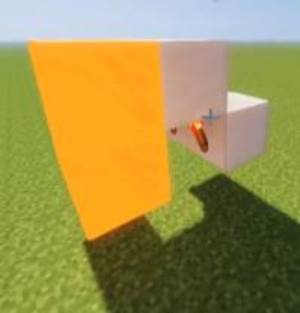
\includegraphics[width=\linewidth]{figures/3a.png}
            \caption{利用两个红石火把控制四个红石灯}
            \label{fig:3a}
        \end{subfigure}
        \hspace{1cm}
        \begin{subfigure}{0.25\linewidth}
            \centering
            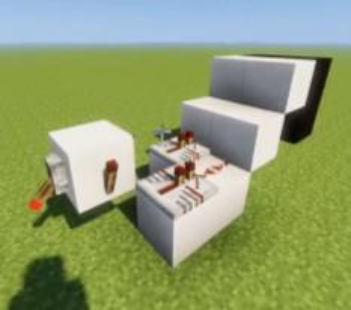
\includegraphics[width=\linewidth]{figures/3b.png}
            \caption{利用拉杆控制红石灯}
            \label{fig:3b}
        \end{subfigure}
        \caption{单个基本显示单元}
        \label{fig:3}
    \end{figure}

    \subsection{RS锁存器}
    清零置位(reset-set, RS)锁存器是一种带有记忆存储功能的模块,其具有一个输出与两个输入,输出与输入之间的关系如表 \ref{tab:2} 所示.

    \begin{table}[H]
        \begin{tabular}{c c c}
        \hlineB{3}
        输入 & 功能 \\
        \hlineB{3}
        清零(置0) & 激活后将输出变为0 \\
        \hline
        置位(置1) & 激活后将输出变为1 \\
        \hlineB{3}
        \end{tabular}
        \caption{RS锁存器的输入}
        \label{tab:2}
    \end{table}

    每个基本显示单元都与一个RS锁存器相连,激活置位端即可点亮像素,激活清零端即可熄灭像素.所有显示单元的清零输入连接至统一的清零信号上,而置位输入则由与门网络分别控制.在我的世界中连接了RS锁存器的基本显示单元如图 \ref{fig:4} 所示.

    \begin{figure}[H]
        \centering
        \begin{subfigure}{0.25\linewidth}
            \centering
            
\includegraphics[width=\linewidth]{figures/4a.png}
            \caption{RS 锁存器与显示单元相连}
        \end{subfigure}
        \hspace{1cm}
        \begin{subfigure}{0.3\linewidth}
            \centering
            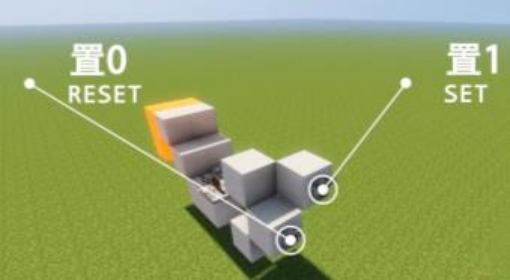
\includegraphics[width=\linewidth]{figures/4b.png}
            \caption{RS锁存器的清零(置0)与置位(置1)输入}
        \end{subfigure}
        \caption{与基本显示单元相连的RS 锁存器相连}
        \label{fig:4}
    \end{figure}

    \subsection{与门网络}
    与门网络内部包括$N^2$个与门,共有$2 N$个输入($N$个列输入与$N$个行输入)和$N^2$个输出,对于输入我们认为未激活的红石信号为1(即被选中),对于输出我们则认为激活的红石火把为1(即被选中),则第$i$行第$j$列的输出等于第$i$个行输入与第$j$个列输入相与.

    列输入与行输入均为独热码形式,即同一时刻各自只会有至多一个信号为1,为1的行或列即为被选中的行或列(即同时只能至多选中一行一列),因此同一时刻输出也至多有一个被选中.

    \begin{figure}[b]
        \centering
        
\includegraphics[width=0.25\linewidth]{figures/5.png}
        \caption{与门网络中的单个与门}
        \label{fig:5}
    \end{figure}

    为了方便控制输入的时刻,防止信号变化过程中误激活错误的像素,我们还可以再加入一个输入控制信号与行列选择信号相与,这样只有当输入控制信号被激活时才会有输出被激活.我的世界中一种与门的建造方法如图 \ref{fig:5} 所示,这种与门可以进行堆叠组成与门网络,如图 \ref{fig:6} 所示.

    \begin{figure}[H]
        \centering
        \begin{subfigure}{0.5\linewidth}
            \centering
            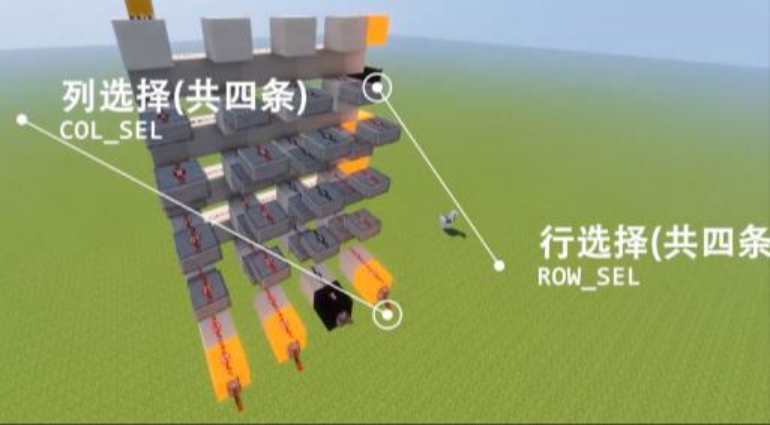
\includegraphics[width=\linewidth]{figures/6a.png}
            \caption{与门网络的输入侧}
        \end{subfigure}
        \hspace{1cm}
        \begin{subfigure}{0.2\linewidth}
            \centering
            
\includegraphics[width=\linewidth]{figures/6b.png}
            \caption{与门网络的输出侧}
        \end{subfigure}
        \caption{$4 \times 4$与门网络}
        \label{fig:6}
    \end{figure}

    \subsection{译码器}
    译码器的功能是将$n$位的二进制行列选择信号分别转换为$N$位的独热码信号,每一条独热码线路都将对应一个唯一的二进制编码,当且仅当二进制码与输入与该条独热码线路对应的编码对应时,该独热码线路被选中.表 \ref{tab:3} 给出了一种2位二进制码与4位独热码之间的对应关系,表中数码转换的译码器被称为2-4译码器.

    \begin{figure}[H]
        \begin{floatrow}
            \ttabbox
            {
                \caption{一种2位二进制码与4位独热码的对应关系}
                \label{tab:3}
            }
            {
                \begin{tabular}{c c c}
                \hlineB{3}
                二进制码 & 独热码 \\
                \hlineB{3}
                00 & 0001 \\
                \hline
                01 & 0010 \\
                \hline
                10 & 0100 \\
                \hline
                11 & 1000 \\
                \hlineB{3}
                \end{tabular}
            }
            \ffigbox
            {
                \caption{2-4译码器中的单个单元}
                \label{fig:7}
            }
            {
                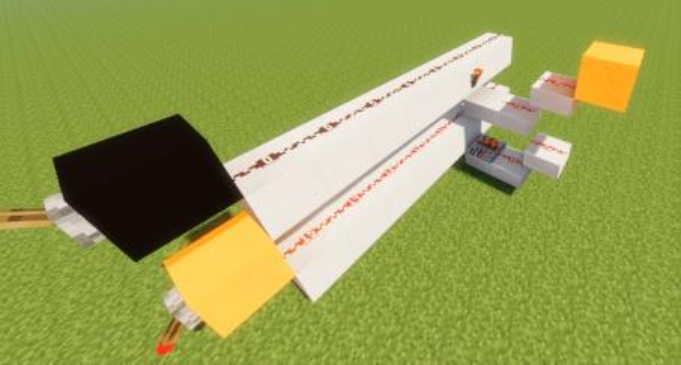
\includegraphics[width=0.7\linewidth]{figures/7.png}
            }
        \end{floatrow}
    \end{figure}

    我的世界中2-4译码器的一个单元的建造方法如图 \ref{fig:7} 所示,其中左侧的两个拉杆为输入(激活时为1),右侧的红石灯为输出(激活时为0),由于右侧红石灯连接到上方线路的红石火把与下方线路的红石中继器上,因此只有当输入为10时,该输出才是1,即该输出对应的是独热码的第3位.

    \section{存储器}
    我们在进行绘图时先将需要绘制的各个点存入存储器内,这里我们使用的是只读存储器(read-only memory, ROM),此类存储器内存出的数据是无法在不改变电路结构的情况下改变的,即无法写入存储数据,因此被称为只读存储器.

    存储器可以被理解为一个包含很多行的表格,存储器的输入为以二进制形式表示的表格的行号,输出则为对应行内存储的信息.存储器每行需要存储$2 n$位的信息(包括$n$位行选择信号与$n$位列选择信号),存储器的总行数取决于存储的点的个数,若共需要在显示器上绘制$M$个点,则存储器共需$M$行空间,同时输入的行号为$m$位二进制,其中$m$满足
    $$2^m \leqslant M < 2^{m+1}$$

    我的世界中的一种存储器的建造方法如图 \ref{fig:8} 所示,右侧的拉杆以独热码形式给出行号信息,存储器将输出激活的行,下方的蓝色线路则是输出,存储器中的内容由图中熄灭的红石火把的位置决定.

    \begin{figure}[H]
        \begin{floatrow}
            \ffigbox
            {
                \caption{存储器}
                \label{fig:8}
            }
            {
                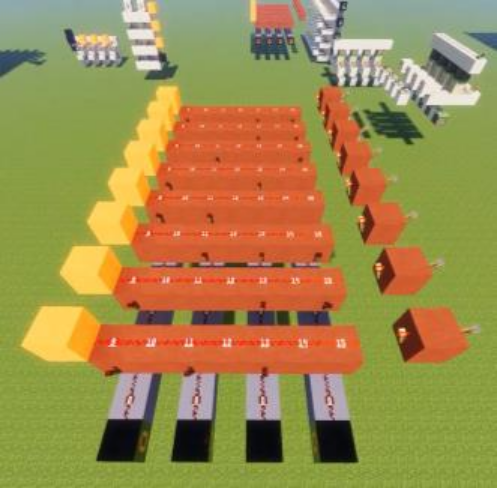
\includegraphics[width=0.5\linewidth]{figures/8.png}
            }
            \ffigbox
            {
                \caption{计数器}
                \label{fig:9}
            }
            {
                
\includegraphics[width=\linewidth]{figures/9.png}
            }
        \end{floatrow}
    \end{figure}

    \section{总控电路}
    \subsection{时钟电路}
    时钟信号可以周期性的发出激活信号,激活信号依次连接到输入控制信号与计数器上,依次将各个点绘制在显示器上.

    \subsection{计数器}
    计数器可以在每次接收到激活信号时将输出加一,计数器的输出连接在存储器的地址输入上,配合时钟信号可以实现依次输出存储器中存储的内容.
    
    我的世界java版中的一种计数器的实现方法如图 \ref{fig:9} 所示,右侧的拉杆为输入,输出由活塞上的各个石英块的高低位置以二进制形式给出.

    \subsection{状态机}
    状态机基于RS锁存器实现,状态机的输出用于控制时钟电路.当RS锁存器输出为0时,时钟信号中断,不再产生激活信号,因此也不会在显示器上输出,RS锁存器输出为1时,时钟电路不断产生激活信号,实现逐个绘图.
    
    状态机的置1端即为显示器的开机信号,置0端则可以与一个计数器输出通过判断逻辑相连,使显示器绘制完固定个数的点后停止显示器的运行.
    
    我的世界中实现总控电路中的状态机与时钟信号的一种方法如图 \ref{fig:10} 所示.

    \begin{figure}[H]
        \centering
        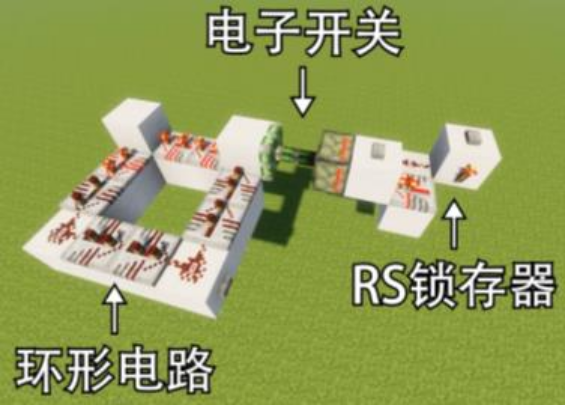
\includegraphics[width=0.25\linewidth]{figures/10.png}
        \caption{总控电路中的时钟线路与状态机}
        \label{fig:10}
    \end{figure}

    \section{结论与展望}
    本文介绍了一种基于基本红石电路的函数绘图显示器,其基本功能是根据设置好的各个点的坐标在显示器中绘制函数图像,文中介绍了显示器各个部分的基本原理.如果在显示器中接入计算元件,也可以显示计算元件得到的函数图像.

    致谢:感谢辰占鳌头的邀稿,让笔者得以在此平台发表自己的拙作;在笔者建造作品的过程中,使用了FredBill提供的整合包,FredBill、辰占鳌头为建造提出了很多建议,很大程度上加快了建造的速度,感谢二位提供的帮助.

    \ds
    \renewcommand{\refname}{参考文献}
    \begin{thebibliography}{99}
        \bibitem{bib:1}辰占鳌头.【Minecraft】全站首个红石汉字编码全像素显示屏 (4K)[V]. Bilibili, BV1wP4y1s7jy.
        \bibitem{bib:2}章鱼千\hspace{-0.015cm}\_zhyq. 【minecraft 红石】6 分钟教你用纯红石电路造一个能打字的大型显示屏[V].Bilibili, BV1Z7411K7a5.
        \bibitem{bib:3}YumNope. 在 我 的 世 界 用 纯 红 石 显 示 屏 做 出 的 bad apple ![V].Bilibili, BV1Je411s7E1.
        \bibitem{bib:4}章鱼千\hspace{-0.015cm}\_zhyq. 【MC 红石】我的世界数电计算器系列教程 1\#:数字显示器[V].Bilibili, BV1Hi4y1877f.
        \bibitem{bib:5}FredBill. MC 红石中的计算机图形学 纯电路 Bresenham 画线机(从零开始搭一台计算机!番外篇) [V].Bilibili, BV1za4y1Y7WS.
    \end{thebibliography}
\end{document}
